\section*{Results}
Associations of Food Groups, Food Subgroups, and Food Nutrients with CKD mortality and ACR as discovered by this study are provided in this section. Also, the impact of Dietary Recommendations Shift on CKD patients  are provided after comparing the recommendations with the findings of this study. 

\subsection*{Food Groups, Food Subgroups, Food Nutrients and CKD Mortality}
\subsubsection*{Food Groups and Mortality}
Experiments with aggregated NHANES and USRDS  data to find associations between food groups and CKD mortality using PCA and Regression show that Grains (-0.84) and Fruits (-0.43) have negative correlations with CKD mortality i.e. mortality is high for the patients who took significantly lower amount of Grains and Fruits than recommended amounts. Data exploration (Figures \ref{foodgroup-negative} ) also reflects the negative relation. As the correlation for fruits is -0.43 i.e. not very high, hence, Fruits can be thought of mildly/moderately associated.
\begin{figure}[!htb]
\small
\begin{tabular}{cc}	
\specialcell{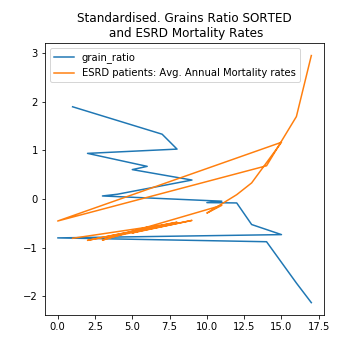
\includegraphics[scale=0.25]{./images/sorted_standard_grain_ratio_negative.png}  }  &  \specialcell{ 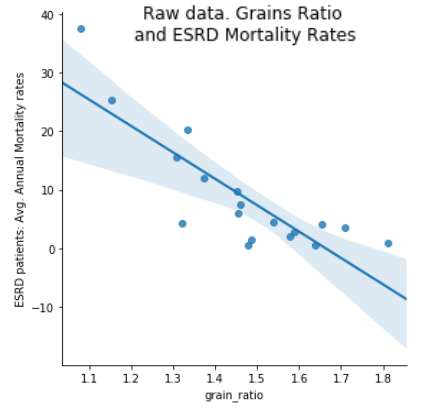
\includegraphics[scale=0.25]{./images/grain_later.png} } \\
Grains & Grains \\
\end{tabular}
\centering
%\vspace{0.25cm}
\begin{tabular}{cc}	
\specialcell{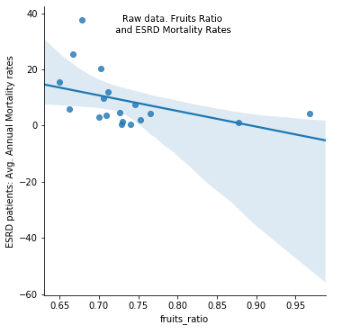
\includegraphics[scale=0.3]{./images/pair_plot_fruits_ratio} } & \specialcell{ 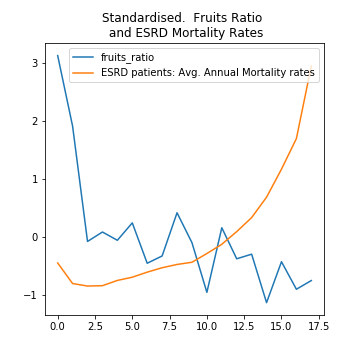
\includegraphics[scale=0.25]{./images/standard_fruit_ratio_mortality.png} } \\
Fruits & Fruits \\
\end{tabular}
\caption{\textbf{Food Groups and Mortality - Negative Correlations}}
%\vspace{0.25cm}
\label{foodgroup-negative}
\end{figure}
\begin{figure}[!htb]
\small
\begin{tabular}{cc}	
	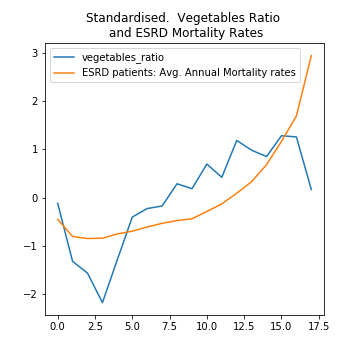
\includegraphics[scale=0.25]{./images/standard_vegetable_ratio.png} & 	
	 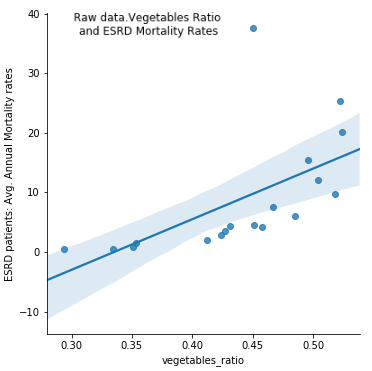
\includegraphics[scale=0.25]{./images/pairplot_vegetable_.png} 	  \\
	\multicolumn{2}{c}{Vegetables Ratio}  \\ 
\end{tabular}
\centering
\caption{\textbf{Food Groups and Mortality - Positive Correlations (Vegetables) }}
\label{vegetable-mortality}
\end{figure}

Vegetables show positive (0.58) correlation i.e. mortality is high for the patients who took more vegetables. The correlation of 0.58 does not provide a very strong conclusion. Data shows such correlations in older adults (Figure \ref{v-subgroup-mortality}). This does not show conformity with the general recommendation to take more vegetables for CKD patients. However, as experiments with food subgroups show that vegetable subgroups such as Other vegetables (0.68), Red and Orange vegetables (0.55), and Starchy vegetables (0.44) show positive correlations that have an impact on the Vegetable group correlation.  Data Exploration plots for Vegetable subgroups as shown in Figure \ref{v-subgroup-mortality} show these positive relations.

 Food subgroups such as Alcoholic Beverages (-0.79),    Added Sugars/Sugars and Sweets (-0.64), Whole Grains (-0.61), and  `Nuts, Seeds, and Soy Products' (-0.55) show the most negative correlations with CKD mortality. Data exploration (Figure \ref{alcohol-sugar-nut} ) also shows negative correlations as shown in the charts below. These outcomes are also consistent with current knowledge except for Sugars. Prevalence of Stage 3 CKD is lower in Alcohol Drinkers than non-drinkers \cite{Jaimonetal2017} \cite{Hsuetal2013}, Nuts being Phosphorus rich and Whole Grains being Potassium rich are detrimental to CKD patients and can cause higher mortality when taken in higher quantities.

\begin{figure}[!htb]
\small
\begin{tabular}{cc}
	\specialcell{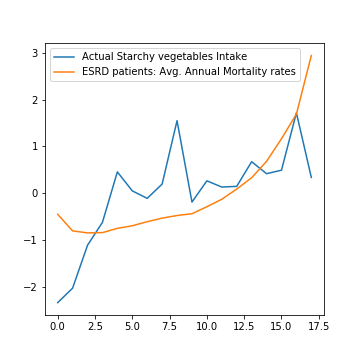
\includegraphics[scale=0.25]{./images/standard_actual_starchy_vegetable_esrd_mortality.png} \\  Starchy Vegetables } & 
	\specialcell{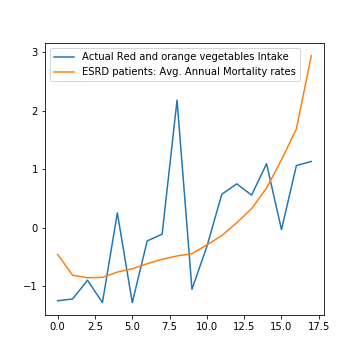
\includegraphics[scale=0.25]{./images/standard_actual_red_and_orange_vegetable_esrd_mortality.png} \\ Red and Orange Vegetables } \\
	 \multicolumn{2}{c} { \specialcell{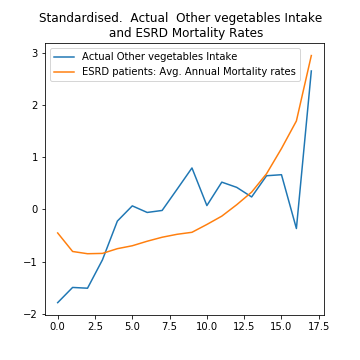
\includegraphics[scale=0.25]{./images/standard_actual_other_vegetable_esrd_mortality.png}	\\ Other Vegetables } } \\
\end{tabular}
\centering
\caption{\textbf{Food Subgroups and Mortality - Positive Correlations}}
\label{v-subgroup-mortality}
\begin{tabular}{cc}
	\specialcell{ 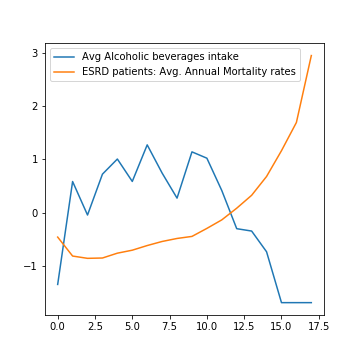
\includegraphics[scale=0.25]{./images/negatively_subgroup_avg_alcohol_intake}  \\   Alcohol Intake  }  & 
	\specialcell{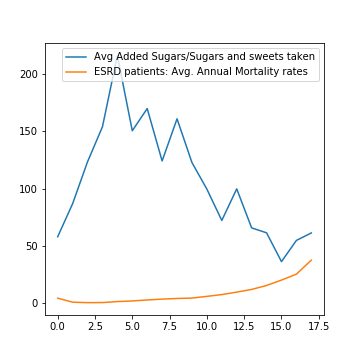
\includegraphics[scale=0.25]{./images/negatively_added_sugar_subgroup_line_2}   \\  Sugar }  \\	
	\specialcell{ 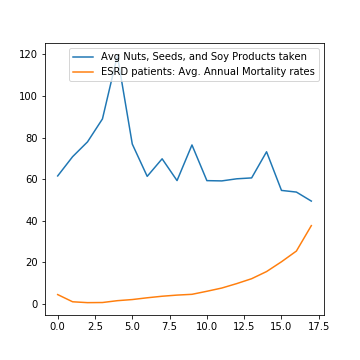
\includegraphics[scale=0.25]{./images/negatively_avg_nuts_subgroup_line_3}  \\ Nuts, Seeds } &
	\specialcell{ 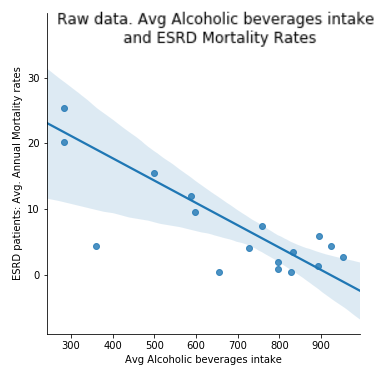
\includegraphics[scale=0.25]{./images/pairplot_avg_alc.png}  \\ Alcohol } \\	
	\specialcell{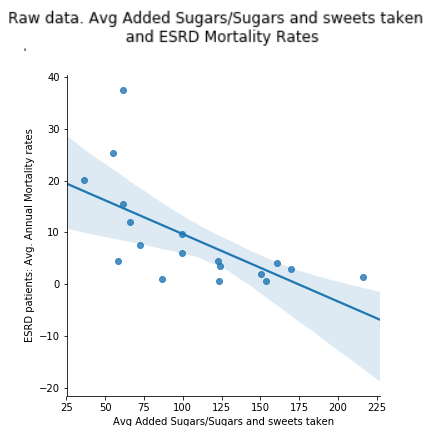
\includegraphics[scale=0.25]{./images/pairplot_raw_data_added_sugar_esrd}  \\ Added Sugar } &
	\specialcell{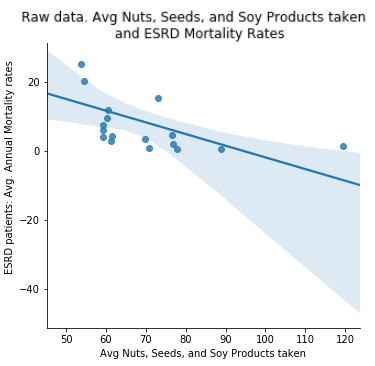
\includegraphics[scale=0.25]{./images/pairplot_nuts_avg_negative.png}  \\ Nuts, Seeds } \\
\end{tabular}
\centering
\caption{\textbf{Food Subgroups and Mortality - Negative Correlations}}
\label{alcohol-sugar-nut}
\end{figure}

\subsubsection*{Mortality Study with Non-aggregated Data}
For experiments where mortality rates based on ages were used for each NHANES survey row (i.e. not aggregated), the following food subgroups show more positive correlations than others: Fats, Eggs, Other vegetables, Nonalcoholic beverages, White potatoes and Puerto Rican starchy vegetables, Tomatoes and tomato mixtures, Oils, Deep-yellow vegetables respectively. In the study, the following subgroups showed more negative correlations than others: Grain mixtures, Frozen plate meals, Soups, Crackers and Salty snacks from grain products, Milks and milk drinks, Sandwiches with Meat, Poultry, and fish, Poultry. Although the correlation numbers in this study are very low, the positive and negative correlations are consistent with current knowledge \cite{Hsuetal2013} \cite{Fernandez-Pradoetal2017} \cite{RippeAngelopoulos2016} \cite{KaraliusShoham2013} \cite{Jaimonetal2017} \cite{Jilian2018} \cite{NKF2019} \cite{Ueharaetal2016} \cite{Nettletonetal2008} \cite{Jacobsetal2009}.

\subsubsection*{Food Groups, Food Nutrients, and Albumin to Creatinine Ratio (ACR) Association}
The experiments using PCA and Regression showed negligible correlation between ACR and food groups and subgroups intake. However, some food groups and/or nutrients such as Dairy, and  `Sugars, Sweets, and Beverages'  have higher and positive though negligible (0.02) effect than the others where Fruits (-0.01) showed negative effect.  For nutrients, Polyunsaturated fatty acids (-0.02), and Iron (-0.02) have negative correlations where Choline (0.02) showed better positive correlation than others. Findings for Choline matches with medical knowledge      \cite{Fernandez-Pradoetal2017} . As the correlations are not significant further analysis can be done on the data especially for food groups and nutrients that are found important (using PCA):

\subsection*{Food Subgroups and Albumin to Creatinine Ratio (ACR) Association}
The experiments showed  `Milk desserts, Sauces, Gravies' (0.22), and Alcoholic Beverages (0.087) have more positive correlations with ACR than the other food subgroups  i.e. taking more of these food subgroups results higher ACR values. Research by Uehara et al. \cite{Ueharaetal2016} also shows that excessive Alcohol consumption can cause Proteinuria/Albuminuria (high ACR). Nettleton et al. \cite{Nettletonetal2008} found that high fat dairy can be linked to high ACR values where low-fat dairy is not strongly linked to high ACR values. However, the correlation as this research found is very low. Low values might still explain a correlation where ACR values might depend on other factors in together than only these food subgroups. Fruits and juicy baby foods show negative correlation (-0.04) though not significant i.e. taking high amount does not increase ACR values that matched with current knowledge \cite{Jacobsetal2009}.